%nohup zathura ./build/notes.pdf > /dev/null &

\documentclass{article}
\usepackage[a4paper]{geometry}
\usepackage{amsmath}
\usepackage{tikz}

\begin{document}

\section{Twice example}

\subsection{Model}

\begin{center}
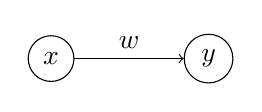
\begin{tikzpicture}
\node[shape=circle, draw=black] (X) at (-1, 0) {$x$};
\node[shape=circle, draw=black] (Y) at (1, 0) {$y$};
\draw[->] (X) -- node[above] {$w$} (Y);
\end{tikzpicture}
\end{center}

\begin{align*}
y = x \cdot w
\end{align*}

\subsection{Cost}

\begin{align*}
C &= \frac{1}{n} \sum _{i=1} ^{n} \left( x_i w - y_i \right) ^2\\
\frac{dC}{dw} &= \frac{d}{dw} \left( \frac{1}{n} \sum _{i=1} ^{n} \left( x_i w - y_i \right) ^2 \right)\\
&= \frac{1}{n} \frac{d}{dw} \left( \sum _{i=1} ^{n} \left( x_i w - y_i \right) ^2 \right)\\
&= \frac{1}{n} \sum _{i=1} ^{n} \frac{d}{dw} \left( \left( x_i w - y_i \right) ^2 \right)\\
&= \frac{1}{n} \sum _{i=1} ^{n} 2 \left( x_i w - y_i \right) x_i\\
\end{align*}

\section{Gates example}

\subsection{Model}

\begin{center}
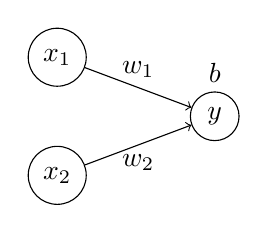
\begin{tikzpicture}
\node[shape=circle, draw=black] (X1) at (-1, 0) {$x_1$};
\node[shape=circle, draw=black] (X2) at (-1, -1.5) {$x_2$};
\node[shape=circle, draw=black] (Y) at (1, -0.75) {$y$};
\node at (1, -0.2) {$b$};
\draw[->] (X1) -- node[above] {$w_1$} (Y);
\draw[->] (X2) -- node[below] {$w_2$} (Y);
\end{tikzpicture}
\end{center}

\begin{align*}
&y = \sigma(x_1 w_1 + x_2 w_2 + b)\\
&\sigma(x) = \frac{1}{1 + e^{-x}}\\
&\frac{d}{dx}\sigma(x) = \sigma(x)(1 - \sigma(x))
\end{align*}

\subsection{Cost}

\begin{align*}
a_i &= \sigma(x_{1i} w_1 + x_{2i} w_2 + b)\\
%
\frac{\partial a_i}{\partial w_1} &= \sigma(x_{1i} w_1 + x_{2i} w_2 + b)(1 - \sigma(x_{1i} w_1 + x_{2i} w_2 + b))x_{1i}\\
&= a_i(1 - a_i)x_{1i}\\
%
\frac{\partial a_i}{\partial w_2} &= \sigma(x_{1i} w_1 + x_{2i} w_2 + b)(1 - \sigma(x_{1i} w_1 + x_{2i} w_2 + b))x_{2i}\\
&= a_i(1 - a_i)x_{2i}\\
%
\frac{\partial a_i}{\partial b} &= \sigma(x_{1i} w_1 + x_{2i} w_2 + b)(1 - \sigma(x_{1i} w_1 + x_{2i} w_2 + b))\\
&= a_i(1 - a_i)\\
%
C &= \frac{1}{n} \sum _{i=1} ^{n} \left( a_i - y_i \right) ^2\\
%
\frac{\partial C}{\partial w_1} &= \frac{\partial}{\partial w_1} \left( \frac{1}{n} \sum _{i=1} ^{n} \left( a_i - y_i \right) ^2 \right)\\
&= \frac{1}{n} \frac{\partial}{\partial w_1} \left( \sum _{i=1} ^{n} \left( a_i - y_i \right) ^2 \right)\\
&= \frac{1}{n} \sum _{i=1} ^{n} \frac{\partial}{\partial w_1} \left( \left( a_i - y_i \right) ^2 \right)\\
&= \frac{1}{n} \sum _{i=1} ^{n} 2(a_i - y_i)a_i(1 - a_i)x_{1i}\\
%
\frac{\partial C}{\partial w_2} &= \frac{\partial}{\partial w_1} \left( \frac{1}{n} \sum _{i=1} ^{n} \left( a_i - y_i \right) ^2 \right)\\
&= \frac{1}{n} \frac{\partial}{\partial w_1} \left( \sum _{i=1} ^{n} \left( a_i - y_i \right) ^2 \right)\\
&= \frac{1}{n} \sum _{i=1} ^{n} \frac{\partial}{\partial w_1} \left( \left( a_i - y_i \right) ^2 \right)\\
&= \frac{1}{n} \sum _{i=1} ^{n} 2(a_i - y_i)a_i(1 - a_i)x_{2i}\\
%
\frac{\partial C}{\partial b} &= \frac{\partial}{\partial w_1} \left( \frac{1}{n} \sum _{i=1} ^{n} \left( a_i - y_i \right) ^2 \right)\\
&= \frac{1}{n} \frac{\partial}{\partial w_1} \left( \sum _{i=1} ^{n} \left( a_i - y_i \right) ^2 \right)\\
&= \frac{1}{n} \sum _{i=1} ^{n} \frac{\partial}{\partial w_1} \left( \left( a_i - y_i \right) ^2 \right)\\
&= \frac{1}{n} \sum _{i=1} ^{n} 2(a_i - y_i)a_i(1 - a_i)\\
\end{align*}

\subsection{Cost - Simplified}

\begin{align*}
a_i &= \sigma(x_{1i} w_1 + x_{2i} w_2 + b)\\
%
\frac{\partial a_i}{\partial w_j} &= a_i(1 - a_i)x_{ji}\\
%
\frac{\partial a_i}{\partial b} &= a_i(1 - a_i)\\
%
C &= \frac{1}{n} \sum _{i=1} ^{n} \left( a_i - y_i \right) ^2\\
%
\frac{\partial C}{\partial w_j} &= \frac{1}{n} \sum _{i=1} ^{n} 2(a_i - y_i)a_i(1 - a_i)x_{ji}\\
%
\frac{\partial C}{\partial b} &= \frac{1}{n} \sum _{i=1} ^{n} 2(a_i - y_i)a_i(1 - a_i)\\
\end{align*}

\end{document}
